\documentclass[tikz]{standalone}
\usepackage{pgfplots}
\usepackage{mathpazo}
\usepgfplotslibrary{polar}
\usepgflibrary{shapes.geometric}
\usetikzlibrary{calc}
\usetikzlibrary{datavisualization}
\usetikzlibrary{datavisualization.formats.functions}
\pgfplotsset{compat=1.12} 
\pgfplotsset{my style/.append style={axis x line=middle, axis y line=middle, xlabel={$x$},ylabel={$y$},smooth}}
\begin{document}
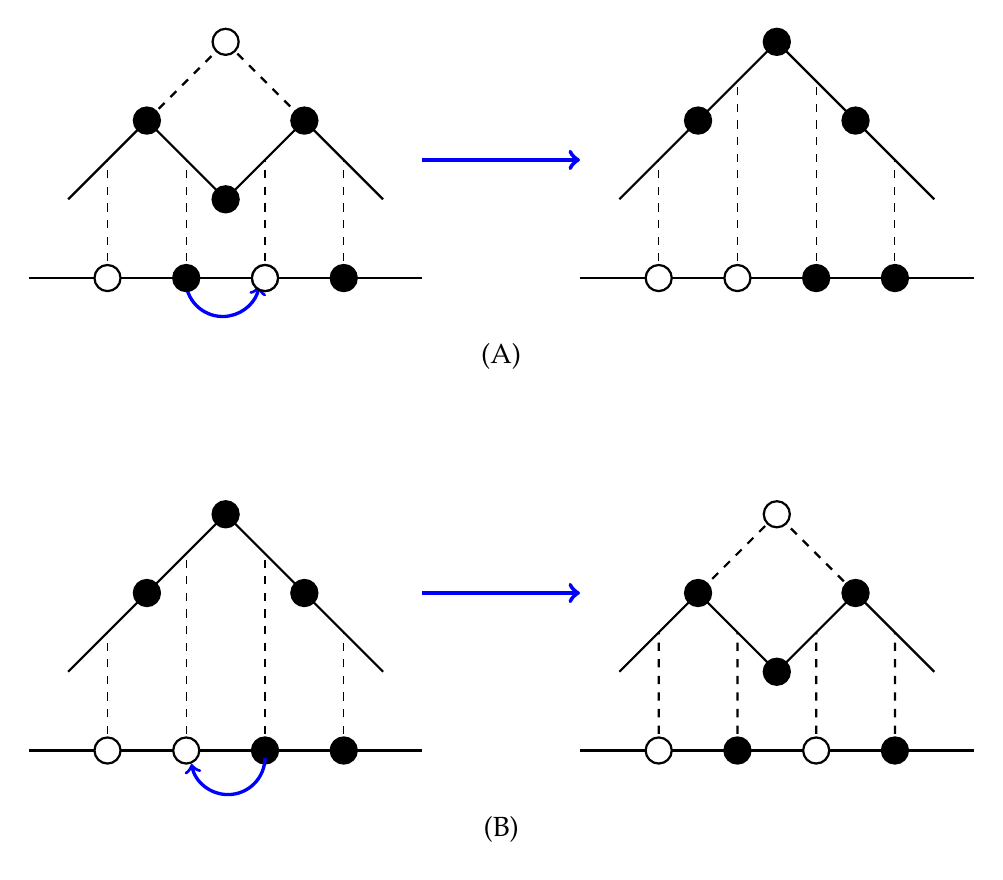
\begin{tikzpicture}[thick]
	%axes
	\draw[thick] (-6, 1) -- (-1, 1);
	\draw (1, 1) -- (6, 1);
	\draw[yshift=1cm] (-6, -6) -- (-1, -6);
	\draw[yshift=1cm] (1, -6) -- (6, -6);
	%A left
	\draw (-5.5, 2) --(-4.5, 3);
	\draw (-4.5, 3) --(-3.5, 2);
	\draw (-3.5, 2) --(-2.5, 3);
	\draw (-2.5, 3) -- (-1.5, 2);
	\draw[dashed, thick] (-4.5, 3) -- (-3.5, 4);
	\draw[dashed] (-3.5, 4) -- (-2.5, 3);
	\draw[dashed, thin] (-5, 1) -- (-5, 2.5);
	\draw[dashed, thin] (-4, 1) -- (-4, 2.5);
	\draw[dashed, thin] (-3, 1) -- (-3, 2.5);
	\draw[dashed, thin] (-2, 1) -- (-2, 2.5);
	\draw[->, very thick,blue] (-4, 0.9) arc [start angle = 190, end angle = 350, radius =0.47];
	%\fill [black] (-5, 1) circle (2pt);
	%\fill [white,opacity=0.5] (-4, 1) circle (2pt);
	\draw 
			(-5, 1) node [fill=white,circle,minimum size=1pt,draw]{}
			(-4, 1) node [fill=black,circle,minimum size=1pt,draw]{}
			(-3, 1) node [fill=white,circle,minimum size=1pt,draw]{}
			(-4.5, 3) node [fill=black,circle,minimum size=1pt,draw]{}
			(-3.5, 2) node [fill=black,circle,minimum size=1pt,draw]{}
			(-2.5, 3) node [fill=black,circle,minimum size=1pt,draw]{}
			(-3.5, 4) node [fill=white,circle,minimum size=1pt,draw]{}
			(-3, 1) node [fill=white,circle,minimum size=1pt,draw]{}
			(-2, 1) node [fill=black,circle,minimum size=1pt,draw]{};
	\draw[blue, ultra thick,->] (-1, 2.5) -- (1, 2.5);
	%A right 
	\draw (5.5, 2) --(4.5, 3);
	\draw (4.5, 3) --(3.5, 4);
	\draw (3.5, 4) --(2.5, 3);
	\draw (2.5, 3) -- (1.5, 2);
	\draw[dashed, thin] (5, 1) -- (5, 2.5);
	\draw[dashed, thin] (4, 1) -- (4, 3.5);
	\draw[dashed, thin] (3, 1) -- (3, 3.5);
	\draw[dashed, thin] (2, 1) -- (2, 2.5);
	\draw 
			(5, 1) node [fill=black,circle,minimum size=1pt,draw]{}
			(4, 1) node [fill=black,circle,minimum size=1pt,draw]{}
			(3, 1) node [fill=white,circle,minimum size=1pt,draw]{}
			(2, 1) node [fill=white,circle,minimum size=1pt,draw]{}
			(4.5, 3) node [fill=black,circle,minimum size=1pt,draw]{}
			(3.5, 4) node [fill=black,circle,minimum size=1pt,draw]{}
			(2.5, 3) node [fill=black,circle,minimum size=1pt,draw]{};
			%(-3.5, 4) node [fill=white,circle,minimum size=1pt,draw]{}
			%(-3, 1) node [fill=white,circle,minimum size=1pt,draw]{};
	\draw (0, 0) node {(A)};
	%B left
	\draw[yshift = 1cm] (0, -7) node {(B)};
	\draw[yshift = 1cm] (-5.5, -5) --(-4.5, -4)
	 		(-4.5, -4) --(-3.5, -3)
	 		(-3.5, -3) --(-2.5, -4)
	 		(-2.5, -4) --(-1.5, -5);
	\draw[dashed, thin, yshift = 1cm] (-5, -6) -- (-5, -4.5)
	 						 (-4, -6) -- (-4, -3.5)
							 (-3, -6) -- (-3, -3.5)
							 (-2, -6) -- (-2, -4.5);
	\draw[yshift = 1cm] 
			(-5, -6) node [fill=white,circle,minimum size=1pt,draw]{}
			(-4, -6) node [fill=white,circle,minimum size=1pt,draw]{}
			(-3, -6) node [fill=black,circle,minimum size=1pt,draw]{}
			(-2, -6) node [fill=black,circle,minimum size=1pt,draw]{}
			(-4.5, -4) node [fill=black,circle,minimum size=1pt,draw]{}
			(-3.5, -3) node [fill=black,circle,minimum size=1pt,draw]{}
			(-2.5, -4) node [fill=black,circle,minimum size=1pt,draw]{};
	\draw[->, very thick,blue, yshift = 1cm] (-3, -6.09) arc [start angle = 0, end angle = -170, radius =0.47];
	\draw[blue, ultra thick,->,yshift = 1cm] (-1, -4) -- (1, -4);
	% B right
	\draw[yshift = 1cm] (5.5, -5) --(4.5, -4)
	 		(4.5, -4) --(3.5, -5)
	 		(3.5, -5) --(2.5, -4)
	 		(2.5, -4) -- (1.5, -5);
	\draw[dashed, thick, yshift = 1cm] (4.5, -4) -- (3.5, -3);
	\draw[dashed,yshift = 1cm] (3.5, -3) -- (2.5, -4)
	 				 (5, -6) -- (5, -4.5)
					 (4, -6) -- (4, -4.5)
					 (3, -6) -- (3, -4.5)
					 (2, -6) -- (2, -4.5);
	%\draw[->, very thick,blue,yshift=1cm] (-4, 0.9) arc [start angle = 190, end angle = 350, radius =0.47];
	%\fill [black] (-5, 1) circle (2pt);
	%\fill [white,opacity=0.5] (-4, 1) circle (2pt);
	\draw[yshift = 1cm] 
			(5, -6) node [fill=black,circle,minimum size=1pt,draw]{}
			(4, -6) node [fill=white,circle,minimum size=1pt,draw]{}
			(3, -6) node [fill=black,circle,minimum size=1pt,draw]{}
			(2, -6) node [fill=white,circle,minimum size=1pt,draw]{}
			(4.5, -4) node [fill=black,circle,minimum size=1pt,draw]{}
			(3.5, -3) node [fill=white,circle,minimum size=1pt,draw]{}
			(2.5, -4) node [fill=black,circle,minimum size=1pt,draw]{}
			(3.5, -5) node [fill=black,circle,minimum size=1pt,draw]{};
\end{tikzpicture}
\end{document}